% This is the chapter 'Model V1.0' to the "Hodgkin-Huxley neuron model V2.0 book"
% Last edited 2026.08.08


\ifx\magyar\undefined
\chapter[The V1.0 model]{The Hodkin-Huxley model (V1.0)}
\else
\chapter[A V1.0 modell]{A  Hodkin-Huxley model (V1.0)} 
\fi
\label{sec:Modell1}

\iflatexml
\else
\minitoc
\fi

\quotationbox{
This was how — Richard P. Feynman approached all knowledge: What can I know for sure, and how can I come to know it?
It resulted in his famous quote, “\textit{You must not fool yourself, and you are the easiest person to fool.}”
}
\index{Feynman, Richard P.}


\ifx\magyar\undefined
\begin{figure}
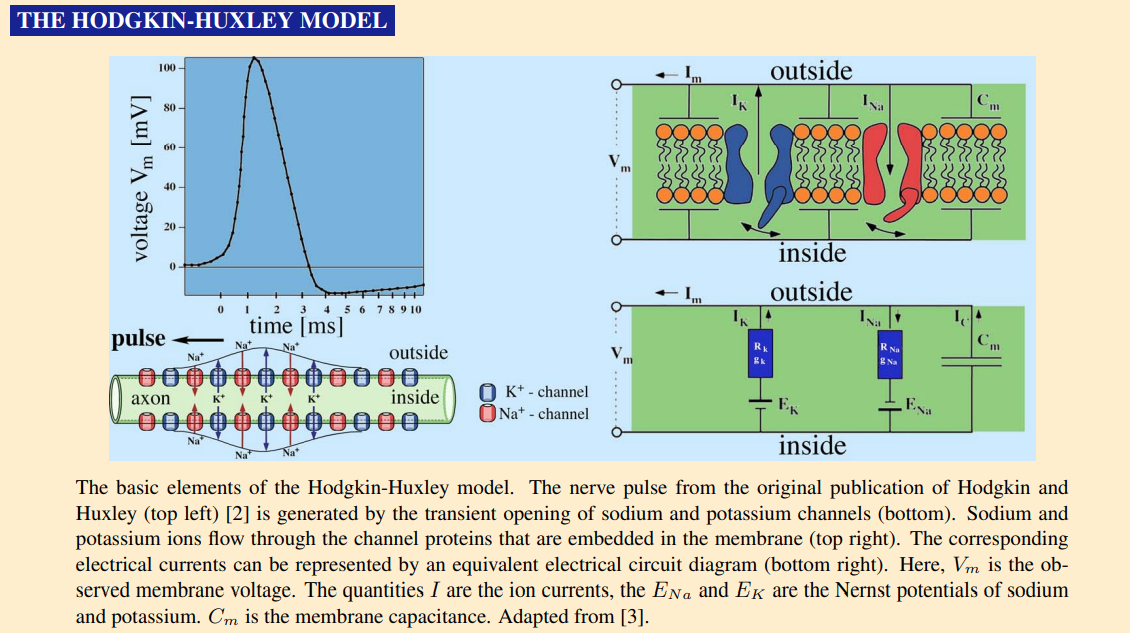
\includegraphics[width=.65\textwidth]{fig/HHModelHeimburg}
\caption{\label{fig:HHModelHeimburg}
The time course of the electric gradient perfectly matches that of the mechanical and thermal changes; however, classic theory cannot explain the connection between them [4]. See Fig.~\ref{fig:HHGradient} how the phase diagram of the voltage change in the function of its gradient matches the experimentally measured values.}	
\end{figure}

\else

\begin{figure}[H]
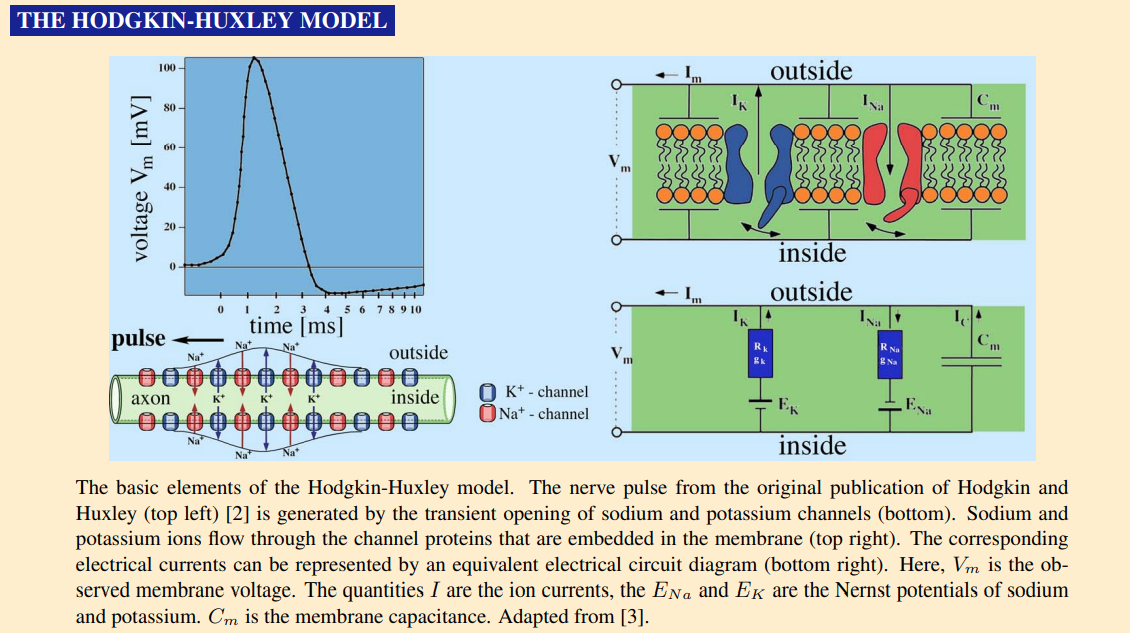
\includegraphics[width=.65\textwidth]{fig/HHModelHeimburg}
\caption{\label{fig:HHModelHeimburg}
The time course of the electric gradient perfectly matches that of the mechanical and thermal changes; however, classic theory cannot explain the connection between them [4]. See Fig.~\ref{fig:HHGradient} how the phase diagram of the voltage change in the function of its gradient matches the experimentally measured values.}	
\end{figure}

\fi

%%The classic model (see Fig.~\ref{fig:HHModelHeimburg}) describes it, but cannot explain why AP is generated, why ion channels open and close, how they are controlled, and how constant batteries create a potential wave [17]. Compare this to the movement in the explained field in Fig. 3 and the voltage change in Fig. 4.


\ifx\magyar\undefined

\proconpanel
{Hodgkin-Huxley V1.0}
{Goods
\begin{itemize}[noitemsep]
	\item 1
	\item 2
\end{itemize}
}
{bads}
\else
{Hodgkin-Huxley V1.0}
{Előny
\begin{itemize}[noitemsep]
	\item 1
	\item 2
\end{itemize}
}
{Hátrány}

\fi


\ifx\magyar\undefined
\section{Equivalent electrical circuit\label{sec:Model1-EquivalentCircuit}}
\else
\section{Ekvivalen áramkör\label{sec:Fallacies-E{sec:Model1-EquivalentCircuit}}}
\fi


\ifx\magyar\undefined

"These ionic concentration gradients across the cell membrane
constitute the driving forces (or chemical potentials)
for ionic currents flowing through open channels in the membrane.
In other words, the ionic concentration gradients act like DC batteries
for cross-membrane currents.”~\cite{JohnstonWuNeurophysiology:1995}

\else

"These ionic concentration gradients across the cell membrane
constitute the driving forces (or chemical potentials)
for ionic currents flowing through open channels in the membrane.
In other words, the ionic concentration gradients act like DC batteries
for cross-membrane currents.”~\cite{JohnstonWuNeurophysiology:1995}

\fi


\ifx\magyar\undefined
Fig.~\ref{fig:AP_schematic} shows the concept 
of the \gls{AP}

\else

A~\ref{fig:AP_schematic} ábrán látható az \gls{AP} elvi menete.
\fi

\ifx\magyar\undefined
\begin{figure}
\centering
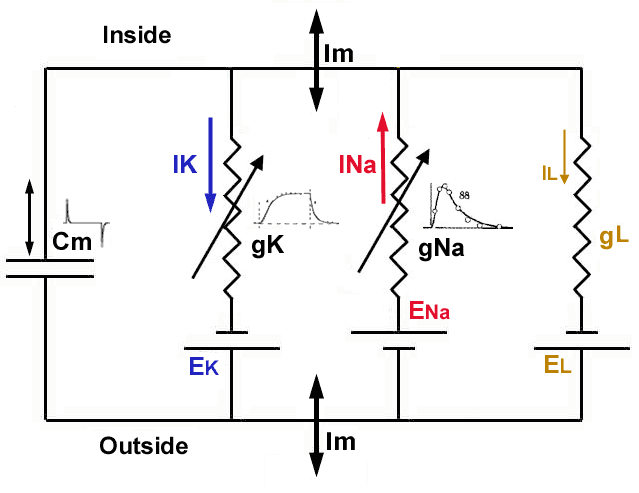
\includegraphics[width=.65\textwidth]{fig/HHcirdiagm.png} 
\caption{The equivalent circuit for the Hodgkin-Huxley model}
\label{fig:HH_EquivalentCircuit}
\end{figure}

\else

\begin{figure}
\centering
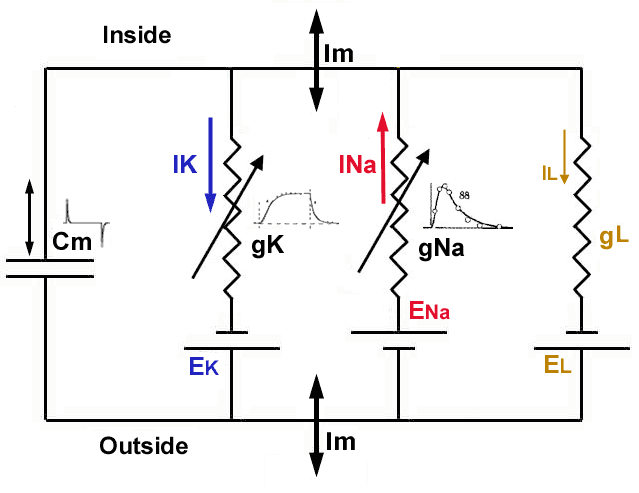
\includegraphics[width=.65\textwidth]{fig/HHcirdiagm.png} 
\caption{A Hodgkin-Huxley modell "ekvivalens áramköre"}
\label{fig:HH_EquivalentCircuit}
\end{figure}

\fi


\ifx\magyar\undefined
The biological 'equivalent circuit' models assume that the circuits comprise point-like
ideal \textit{discrete elements}
such as condensers and resistors, and some hidden power changes their parameters according to some
mathematical formulas,
furthermore ideal batteries with voltage that may again be changed  by that power.
All they are connected by conducting  (metallic) ideal wires
and their interaction speed is infinitely high (the Newtonian 'instant interaction').
Using that abstract model enables them to use the well-known classic equations, named after
Ohm, Kirchoff, Coulomb, Maxwell and others. However, those abstractions have severe limitations.
Biology applies Ohm's Law to its objects while claims that its objects are non-ohmic;
understands that neural currents comprise ions while claims that the ions do not feel the Coulomb repulsion;
measures ions' propagation speed but in its equations it claims that their effects are instant;
hypotesizes non-existing physical mechanisms to make their nature. In general,
biophysics abstracts from the world of the physics-inspired mathematical formulas a fictitious nature
where biology lives and hypothesises complementary mechanisms to achieve some resemblance with the true biological word.
The examples include that ions in the ions channels do not repulse each other;
that charge, potential and current are independent of each other;
that ion currents do not repulse each other neither when they travel from the presynaptic terminal to the
\index{Coulomb's law}
\gls{AIS};
that some hidden power opens the ion channels to let ions in into the intracellular space,
that ions with the same charge move in opposite directions when ions rush-in into the intracellular segment of the neuron;
that the ions pass ion channels without being accelerated by the potential difference accross the membrane;
the telegraph equations are applied to the case of axons although neither external potential nor current loss exists; and so on.


Even that unfortunate idea of equivalent circuits leads to analyzing
"electrotonic (electronic circuit equivalent) modeling of realistic neurons and the interaction of dendritic morphology
and voltage-dependent membrane properties on the processing of neuronal synaptic input"~\cite{SingleNeuronComputation:2014};
that is, to study a simulated neuron built from discrete electronic components. However, the idea needs to put together
many compone "raises the possibility that the neuron is itself a network". On the one side, such an idea misguides the neurophysical research (since actually a fake neural system is scrutinized, the validity of the approach is questionalized~\cite{RealisticNeuronalModeling:2016}), and on the other, since electroengineers understand
the neuronal operation from the wrong model, it also misguides building neuromorphic architectures. 

\else

The biological 'equivalent circuit' models assume that the circuits comprise point-like
ideal \textit{discrete elements}
such as condensers and resistors, and some hidden power changes their parameters according to some
mathematical formulas,
furthermore ideal batteries with voltage that may again be changed  by that power.
All they are connected by conducting  (metallic) ideal wires
and their interaction speed is infinitely high (the Newtonian 'instant interaction').
Using that abstract model enables them to use the well-known classic equations, named after
Ohm, Kirchoff, Coulomb, Maxwell and others. However, those abstractions have severe limitations.
Biology applies Ohm's Law to its objects while claims that its objects are non-ohmic;
understands that neural currents comprise ions while claims that the ions do not feel the Coulomb repulsion;
measures ions' propagation speed but in its equations it claims that their effects are instant;
hypotesizes non-existing physical mechanisms to make their nature. In general,
biophysics abstracts from the world of the physics-inspired mathematical formulas a fictitious nature
where biology lives and hypothesises complementary mechanisms to achieve some resemblance with the true biological word.
The examples include that ions in the ions channels do not repulse each other;
that charge, potential and current are independent of each other;
that ion currents do not repulse each other neither when they travel from the presynaptic terminal to the
\index{Coulomb's law}
\gls{AIS};
that some hidden power opens the ion channels to let ions in into the intracellular space,
that ions with the same charge move in opposite directions when ions rush-in into the intracellular segment of the neuron;
that the ions pass ion channels without being accelerated by the potential difference accross the membrane;
the telegraph equations are applied to the case of axons although neither external potential nor current loss exists; and so on.


Even that unfortunate idea of equivalent circuits leads to analyzing
"electrotonic (electronic circuit equivalent) modeling of realistic neurons and the interaction of dendritic morphology
and voltage-dependent membrane properties on the processing of neuronal synaptic input"~\cite{SingleNeuronComputation:2014};
that is, to study a simulated neuron built from discrete electronic components. However, the idea needs to put together
many compone "raises the possibility that the neuron is itself a network". On the one side, such an idea misguides the neurophysical research (since actually a fake neural system is scrutinized, the validity of the approach is questionalized~\cite{RealisticNeuronalModeling:2016}), and on the other, since electroengineers understand
the neuronal operation from the wrong model, it also misguides building neuromorphic architectures. 
\fi

\ifx\magyar\undefined
The equivalent circuits are a source of misinterpretations. As~\cite{JohnstonWuNeurophysiology:1995} formulates,
"In other words, the ionic concentration gradients act like DC batteries for cross-membrane currents."
We call the attention again, that \textit{ions} represent the current,
that is \textit{that current changes changes the concentration, that changes
the voltage of the DC battery, unlike in the case of the equivalent circuits}.
This difference is significant in understand how the basic neuronal circuit works.
Introducing equivalent circuits prevents explaining the fundamental 
electric phenomena.


%\subsection[Equivalent circuits]{Equivalent circuits\label{sec:PHYSICS_EquivalentCircuit}}
%
One wrong consequence of forgetting that the charge transfer mechanism is entirely different,
the charge carriers are large and heavy (and as a consequence: slow) ions instead of electron (cloud),
furthermore they are not necessary present in the 
volume under test and the 'construction' of biological matter 
enables the tested medium to produce charge carriers,
using 'equivalent circuits' for
neuronal operation. This fallacy
entirely falsifies the conclusions from the measurements.

\else

The equivalent circuits are a source of misinterpretations. As~\cite{JohnstonWuNeurophysiology:1995} formulates,
"In other words, the ionic concentration gradients act like DC batteries for cross-membrane currents."
We call the attention again, that \textit{ions} represent the current,
that is \textit{that current changes changes the concentration, that changes
the voltage of the DC battery, unlike in the case of the equivalent circuits}.
This difference is significant in understand how the basic neuronal circuit works.
Introducing equivalent circuits prevents explaining the fundamental 
electric phenomena.


%\subsection[Equivalent circuits]{Equivalent circuits\label{sec:PHYSICS_EquivalentCircuit}}
%
One wrong consequence of forgetting that the charge transfer mechanism is entirely different,
the charge carriers are large and heavy (and as a consequence: slow) ions instead of electron (cloud),
furthermore they are not necessary present in the 
volume under test and the 'construction' of biological matter 
enables the tested medium to produce charge carriers,
using 'equivalent circuits' for
neuronal operation. This fallacy
entirely falsifies the conclusions from the measurements.
\fi


\ifx\magyar\undefined
Another wrong consequence of using 'equivalent circuits' to describe
the electrical operation of neurons is believing that the currents in
the biological circuit do not change the concentration, and through
the concentration, also the potential; see also section~\ref{sec:Physics-Resources}. The 'equivalent circuits',
of course, use a constant potential (they follow the abstraction used
in the theory of electricity, although the 'ideal batteries' also
may produce their voltage using chemical processes), and unreasonably, some mystic process changes the resistance/conductance of components. This wrong abstraction
results in numerous misunderstandings, among others, introducing ideas
such as parallel oscillator equivalent of neuron, input resistance,
delayed rectifier current, resting current, and time- or voltage-dependent
conductance. Furthermore, we cannot 
interpret, among others, \emph{how neuronal electricity
works in lack of external potential}; \emph{how slow currents operate
neuron's infrastructure}, \emph{how and why action potential is generated}.
Deriving the time course of the Nernst-Planck potential opens the
way to a quantitative understanding of neurophysical electrical processes,
including their time course.

Again another wrong consequence is that the two secondary abstractions 'potential',
and 'current', became independent from the primary abstraction 'charge'
and each other (significantly contributing to the fallacy that 'physics cannot describe life'). Our equations and the underlying discussion point
to the fact that \emph{the potential and the current cannot be separated
from the charge}. No 'delayed rectifying current' and 'voltage- (or
time-) dependent conductance' exist. Those notions originate from
the wrong interpretation of measured data derived from mismatching
measured electrical data pairs and the misconception that biological
structures and materials must behave like metals.

\else

Another wrong consequence of using 'equivalent circuits' to describe
the electrical operation of neurons is believing that the currents in
the biological circuit do not change the concentration, and through
the concentration, also the potential; see also section~\ref{sec:Physics-Resources}. The 'equivalent circuits',
of course, use a constant potential (they follow the abstraction used
in the theory of electricity, although the 'ideal batteries' also
may produce their voltage using chemical processes), and unreasonably, some mystic process changes the resistance/conductance of components. This wrong abstraction
results in numerous misunderstandings, among others, introducing ideas
such as parallel oscillator equivalent of neuron, input resistance,
delayed rectifier current, resting current, and time- or voltage-dependent
conductance. Furthermore, we cannot 
interpret, among others, \emph{how neuronal electricity
works in lack of external potential}; \emph{how slow currents operate
neuron's infrastructure}, \emph{how and why action potential is generated}.
Deriving the time course of the Nernst-Planck potential opens the
way to a quantitative understanding of neurophysical electrical processes,
including their time course.

Again another wrong consequence is that the two secondary abstractions 'potential',
and 'current', became independent from the primary abstraction 'charge'
and each other (significantly contributing to the fallacy that 'physics cannot describe life'). Our equations and the underlying discussion point
to the fact that \emph{the potential and the current cannot be separated
from the charge}. No 'delayed rectifying current' and 'voltage- (or
time-) dependent conductance' exist. Those notions originate from
the wrong interpretation of measured data derived from mismatching
measured electrical data pairs and the misconception that biological
structures and materials must behave like metals.
\fi

\ifx\magyar\undefined
As we discussed in section~\ref{sec:Physics-TwoSegments}, 
the unbalanced charge in neurons and the charge injected
suddenly into the intracellular segment during a rush-in action
are in the same order of magnitude. We also discussed that 
the charge injection (the appearance and flow of charge in the proximal layer on the membrane's surface) causes well measureable mechanical, optical, etc. changes~\cite{MechanicalWaves:2015} on the membrane.
Those changes are well observable on the low-concentration side, in the form of slow currents, and large-scale
concentration and potential changes.

Those changes also mean that a large amount of charge
passes from the high-concentration side
to the low concentration side of the membrane, and causes a sudden drop
on the high-concentration side of the membrane. As discussed,
that change means simultaneously a change in the corresponding 
potentials across the membrane that solves the mystery why the
\gls{AP}
AP stops. The potential across the membrane is defined by the difference of the
potential of the two thin layers (see section~\ref{sec:Physics-Membranes}) on the membrane's surface.
As we discussed, a huge electric field exists across the
plates of the neuronal condenser, while a moderate one 
in the proximal layers. That means that the ions can quickly
leave the high concentration when the rush-in injection begins.
They produce an 'empty' layer (and a potential gradient)
whithin that layer and the ions in the neighboring layer
start to move using the 'downhill' potential. However, they do have a much slower speed, so they 'stop' at some distance. 


\else

As we discussed in section~\ref{sec:Physics-TwoSegments}, 
the unbalanced charge in neurons and the charge injected
suddenly into the intracellular segment during a rush-in action
are in the same order of magnitude. We also discussed that 
the charge injection (the appearance and flow of charge in the proximal layer on the membrane's surface) causes well measureable mechanical, optical, etc. changes~\cite{MechanicalWaves:2015} on the membrane.
Those changes are well observable on the low-concentration side, in the form of slow currents, and large-scale
concentration and potential changes.

Those changes also mean that a large amount of charge
passes from the high-concentration side
to the low concentration side of the membrane, and causes a sudden drop
on the high-concentration side of the membrane. As discussed,
that change means simultaneously a change in the corresponding 
potentials across the membrane that solves the mystery why the
\gls{AP}
AP stops. The potential across the membrane is defined by the difference of the
potential of the two thin layers (see section~\ref{sec:Physics-Membranes}) on the membrane's surface.
As we discussed, a huge electric field exists across the
plates of the neuronal condenser, while a moderate one 
in the proximal layers. That means that the ions can quickly
leave the high concentration when the rush-in injection begins.
They produce an 'empty' layer (and a potential gradient)
whithin that layer and the ions in the neighboring layer
start to move using the 'downhill' potential. However, they do have a much slower speed, so they 'stop' at some distance. 
\fi



